% --- SLIDE 14: Bohm & Aharonov ---
\begin{frame}{Bohm \& Aharonov: Simplifying EPR}

  \begin{columns}[T]
    \begin{column}{0.6\textwidth}
      \begin{block}{A clearer, more experimental approach}
        \begin{itemize}[<+->]
          \item In 1951, \textbf{David Bohm} reformulated the EPR paradox in a conceptually clearer way.
          \item Together with \textbf{Yakir Aharonov} (in 1957), they simplified the example from continuous variables to the \textbf{discrete variable of spin}.
          \item This made the thought experiment much more \textbf{amenable to experimental verification}.
        \end{itemize}
      \end{block}
    \end{column}

    \begin{column}{0.4\textwidth}
      \begin{figure}
        \centering
        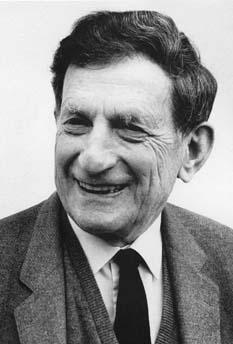
\includegraphics[width=\linewidth, height=0.7\textheight, keepaspectratio]{images/David_Bohm.jpg}
        \caption{David Bohm \cite{fotografo_desconocido_fotografidavid_nodate}.}
      \end{figure}
    \end{column}
  \end{columns}
\end{frame}

% --- SLIDE 15: The Spin Singlet State ---
\begin{frame}{The Spin Singlet State}
  \begin{columns}[T]
    \begin{column}{0.5\textwidth}
      \begin{block}{An example with spin-1/2 particles}
        \begin{itemize}[<+->]
          \item Consider a molecule with total spin zero that decays into two atoms (A and B) with spin 1/2.
          \item It is an \textbf{entangled} state where the total spin is zero, regardless of the measurement axis.
        \end{itemize}
      \end{block}
      \vspace{0.5em}
      The entangled wave function:
      $$ {\Psi} = \frac{1}{\sqrt{2}} \left( \Psi_{+}{(1)} \Psi_{-}{(2)} - \Psi_{-}{(1)} \Psi_{+}{(2)} \right) $$
    \end{column}

    \begin{column}{0.5\textwidth}
      \begin{figure}
        \centering
        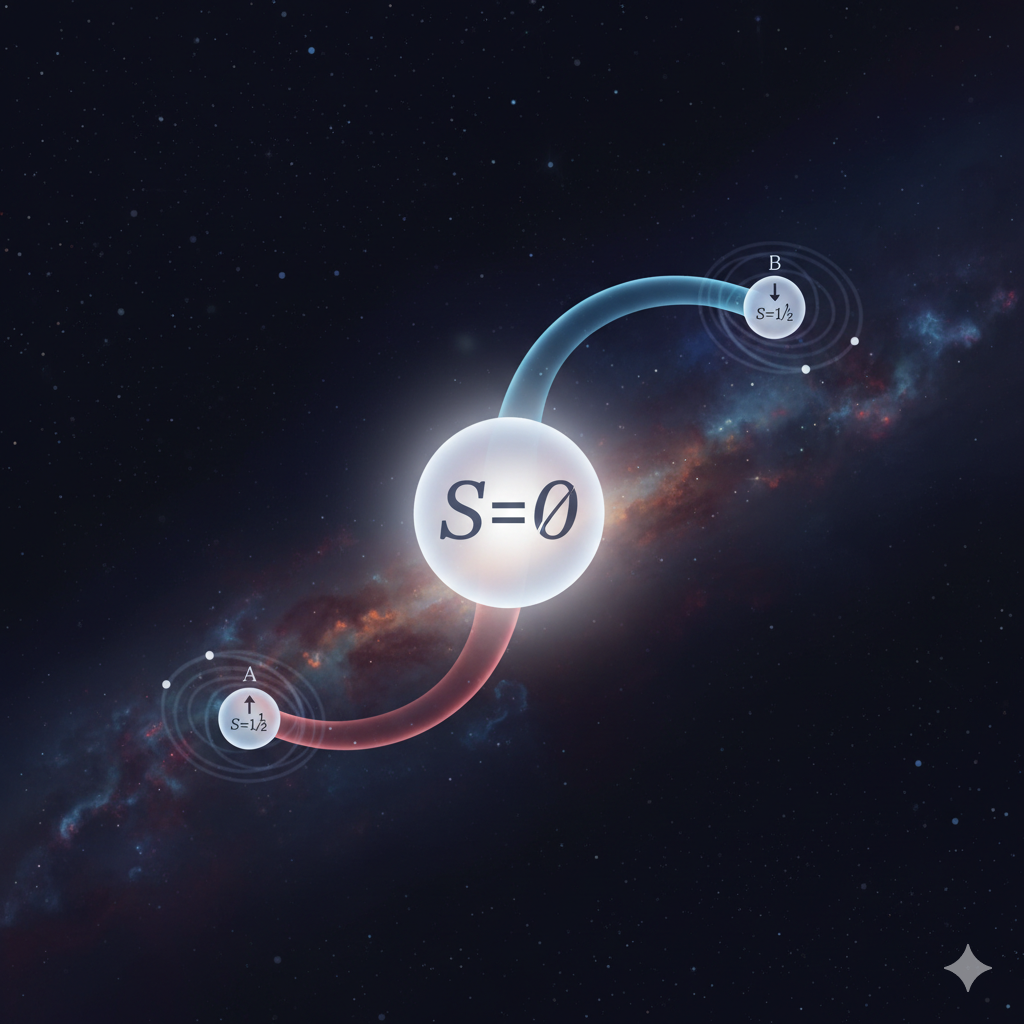
\includegraphics[height=0.7\textheight, keepaspectratio]{images/spin.png}
        \caption{A source emits two entangled particles with opposite spin \cite{google_fuente_2025}.}
      \end{figure}
    \end{column}
  \end{columns}
\end{frame}

% --- SLIDE 16: Classical vs. Quantum ---
\begin{frame}{The Core of the Paradox: Classical vs. Quantum}

  \begin{columns}[T]
    \begin{column}{0.5\textwidth}
      \begin{alertblock}{Classical Interpretation (Local Realism)}
        \begin{itemize}[<+->]
          \item The atoms have \textbf{pre-existing} and perfectly anti-correlated spin vectors.
          \item The measurement on A only \textbf{reveals} an already existing property.
          \item There is no instantaneous influence at a distance; the correlation was established locally at the source.
        \end{itemize}
      \end{alertblock}
    \end{column}

    \begin{column}{0.5\textwidth}
      \begin{block}{Quantum Interpretation}
        \begin{itemize}[<+->]
          \item A particle's spin state is \textbf{not defined until it is measured}.
          \item The choice to measure A's spin \textbf{realizes} its value, and due to entanglement, simultaneously realizes the opposite value for B.
          \item This happens \textbf{instantaneously}, despite the distance, seemingly violating locality.
        \end{itemize}
      \end{block}
    \end{column}
  \end{columns}

  \uncover<7->{
    \textbf{Key conclusion:} Quantum uncertainty in entangled systems is an intrinsic property of the \textbf{non-separable correlations} that define the state of the system as a whole.
  }

\end{frame}

% --- SLIDE 17: Alternative Hypothesis ---
\begin{frame}{The Alternative Hypothesis: Entanglement Breaking}

  \begin{block}{Entanglement that ``decays'' with distance}
    \begin{itemize}[<+->]
      \item The idea is raised that the quantum many-body formulation \textbf{might not be valid} for widely separated particles.
      \item The proposal suggests that entanglement is a phenomenon that \textbf{decreases with distance}.
      \item An alternative \textbf{``classical'' state} is proposed for the system after separation.
    \end{itemize}
  \end{block}
  \uncover<4->{ % The equation appears after the points
    \justifying
    \vspace{0.5em}
    Alternative state (statistical mixture):
    $$ {\Psi} =  \Psi_{+\theta,\phi}{(1)} \Psi_{-\theta,\phi}{(2)}  $$
  }

\end{frame}

% --- SLIDE 18: Consequences and Difference ---
\begin{frame}{Consequences: Quantum Superposition vs. Classical Mixture}

  \begin{block}{Implications of the Breaking Hypothesis}
    \begin{itemize}[<+->]
      \item \textbf{Avoidance of the EPR Paradox:} It restores local realism; the measurement on A only reveals a pre-existing spin direction.
      \item \textbf{Violation of Angular Momentum Conservation:} In individual events, total angular momentum would not be conserved (but it would on average).
      \item This pre-existing spin direction acts as a \textbf{``hidden variable''}.
    \end{itemize}
  \end{block}

  \begin{alertblock}{Crucial Difference: Quantum Superposition vs. Statistical Mixture}
    \begin{itemize}[<+->]
      \item \textbf{Quantum Superposition (Entanglement):} Maintains perfect correlations in \textbf{any} measurement basis.
      \item \textbf{Classical Statistical Mixture:} Only exhibits perfect correlations in the basis defined by the hidden variable.
    \end{itemize}
  \end{alertblock}

\end{frame}

% --- SLIDE 19: Photon Polarization Analogue ---
\begin{frame}{An Experimental Analogue: Photon Polarization}

  \begin{columns}[T]
    \begin{column}{0.6\textwidth}
      \begin{block}{From Spin to Polarization}
        \begin{itemize}[<+->]
          \item A more viable analogue is proposed: the \textbf{polarization} of photons from \textbf{positron-electron annihilation}.
          \item \textbf{Conservation Laws:} Due to conservation of angular momentum and parity, the two emitted photons must have mutually \textbf{perpendicular} polarizations.
        \end{itemize}
      \end{block}
      \vspace{0.5em}
      Wave function of the system:
      $$ {\Phi} = \frac{1}{\sqrt{2}} \left( C_1^x C_2^y - C_1^y C_2^x \right) \Psi_0 $$
    \end{column}

    \begin{column}{0.4\textwidth}
      \begin{figure}
        \centering
        \includegraphics[height=0.7\textheight, keepaspectratio]{images/Aniquilación.png}
        \caption{Scheme of the experiment: a source emits two entangled photons \cite{goole_esquema_2025}.}
      \end{figure}
    \end{column}
  \end{columns}

\end{frame}

% --- SLIDE 20: Wu and Shaknov Experiment ---
\begin{frame}{The Identified Experiment: Wu and Shaknov (1950)}

  \begin{block}{A Reinterpretation of Existing Data}
    \begin{itemize}[<+->]
      \item Bohm and Aharonov did not propose a new experiment, but reinterpreted data already published by \textbf{Chien-Shiung Wu and Irving Shaknov} in 1950.
      \item Their contribution was theoretical: to unveil the fundamental implications of a previously known experimental result.
    \end{itemize}
  \end{block}

  \begin{alertblock}{Measurement Process and Setups}
    \begin{itemize}[<+->]
      \item Polarization is measured indirectly via \textbf{Compton Scattering}.
      \item The rate of \textbf{coincidences} (simultaneous detection of both photons) is measured in two geometries:
        \begin{itemize}
          \item \textbf{Perpendicular} scattering planes ($\varphi = 90^\circ$).
          \item \textbf{Parallel} scattering planes ($\varphi = 0^\circ$).
        \end{itemize}
    \end{itemize}
  \end{alertblock}

\end{frame}

% --- SLIDE 21: The Experimental Verdict ---
\begin{frame}{The Experimental Verdict: The Ratio R}

  \begin{block}{The Crucial Ratio and the Predictions}
    The ratio R is defined as the quotient of the coincidence rates between the two geometries:
    $$ R = \frac{\text{Coincidence Rate}(\text{parallel})}{\text{Coincidence Rate}(\text{perpendicular})} $$
    \begin{itemize}[<+->]
      \item \textbf{Quantum Mechanics Prediction (Entangled State):}
        \begin{itemize}
          \item \textbf{R = 2.00}
        \end{itemize}
      \item \textbf{Local Realism Predictions (Statistical Mixture):}
        \begin{itemize}
          \item Circular Polarization (B1): \textbf{R = 1.00}
          \item Linear Polarization (B2): \textbf{R < 2} (approx. 1.5)
        \end{itemize}
    \end{itemize}
  \end{block}

  \begin{alertblock}{The Experimental Result (Wu, 1950): $R = 2.04 \pm 0.08$}
  \end{alertblock}

\end{frame}
